\subsubsection{\stid{1.08} Legion}

\paragraph{Overview}
This project focuses on the development, hardening and support of the
Legion Programming System with a focus on Exascale platforms and workloads
that can benefit from Legion's features.  At a fundamental level our focus 
is on the key capabilities (e.g. correctness, performance, scalability) of 
an alternative programming model for ECP that seeks to expose additional levels
of parallelism in applications.  In addition, Legion also enables a separation of 
concerns of the implementation of an application from how it is mapped onto a 
given system architecture.  Our efforts are currently focused on addressing bugs, 
refactoring the implementation for improved stability, performance and scaling,
extending support for the selected exascale platforms (Aurora and Frontier), and
also expanding the feature set as needed for both application and platform nuances. 

The Legion Programming System is freely available with an Apache-based
open source license and is hosted at GitLab:

\begin{quote} 
  \url{https://gitlab.com/StanfordLegion/legion}
\end{quote}

\paragraph{Key Challenges}
While Legion addresses a number of key challenges in improving system
utilization and some aspects of platform portability, it is a
relatively new programming system and therefore there is a cost to
rewriting applications.  This aspect makes significant adoption a risk
within ECP and additional effort must also take place to catch up with
aspects of performance and scaling to match aspects of more mature
technologies.

We have recently started to focus much of our efforts on emerging use 
cases that are related to machine learning and data-centric workloads.
These domains are much easier to have a substantial impact as the application
codes rely on external tools (e.g. TensorFlow, Python, etc.) vs. years of 
established code written in MPI and/or OpenMP.  We are already seeing clear 
benefits of focusing our efforts in this direction. This has helped us to 
increase our overall impact as well focus on areas of adoption 
across more specialized application needs in support of machine learning 
and other data-centric workloads. 

\paragraph{Solution Strategy}
As a collaboration between Los Alamos, Stanford University and other
efforts at NVIDIA and SLAC, we are providing the overarching
implementation Legion programming model that captures the ``best''
(correct and feature complete) version of the code.  In addition, we
are actively looking for opportunities to educate the ECP community
about Legion and other data-centric and task-based approaches to
programming.  Most recently we have been closely working with ExaFEL (AD
2.2.4.05) and the CANDLE project (AD 2.2.4.03) to provide support for 
Legion.  We also provide support and software releases related to the 
efforts going on within LANL's ATDM Programming Models and Runtimes 
project (part of ST 2.3.6.01), that refine, identify needs and requirements that
are in support of Ristra (LANL's National Security application AD 2.2.5.01). 
Our project includes management of the current repository and quarterly, 
or more frequent, releases of Legion to the broader community.  We are also 
looking at numerous aspects of having the Legion system interoperate with 
today's more widely used programming systems -- e.g. MPI and OpenMP. 

More recently we have started to look at leveraging recent results in 
improving the performance of training deep learning applications.  Our 
most recent results explore CANDLE's requirements for ML training and 
inference on large DNNs. This is discussed in more detail below. 

Finally, we are actively exploring techniques to simplify Legion
programming and improve overall developer productivity.  This has been a 
both a broader community effort that focuses on both connections with 
Python (e.g. see ~\cite{2.3.1.08:Bauer:2019} and ~\cite{2.3.1.08:Slaughter:2019}) 
and also furthering the development and performance of 
FlexFlow~\cite{2.3.1.08:Jia:2018:2} by looking at the impact of performance
improvements to Legion such as the work in~\cite{2.3.1.08:Lee:2018:1}. 


\paragraph{Recent Progress}
As discussed above, our progress to date has been focused improving 
training times for CANDLE's DNN use cases.  For example, training a 
single epoch of the Uno dataset (with 21 million samples) using TensorFlow 
requires 27 hours on 1 GPU and 18 hours on 3 GPUs (where it reaches a 
scalability limit for TensorFlow).  Using FlexFlow, a deep learning
framework built on top of Legion, the training time is reduced to 1.2 hours on 
128 Summit nodes, using 768 GPUs. This represents a 15x speedup and as 
shown in Figure~\ref{fig:2.3.2.08:flexflow} has significantly better scaling 
than TensorFlow.

In addition to the these efforts we continue to focus on bug fixes, performance 
improvements and overall scalability. We have also started to address exascale 
platform-centric details and have started to work on targeting AMD's software 
infrastructure for Frontier and are beginning to explore the details of Intel's software 
stack for Aurora. In addition, we have started to diversify and modularize 
the low-level transport layers of the system to use both GASNetEX 
(ST 2.3.1.14) and a modern MPI layer (ST 2.3.1.07). This approach will 
give us multiple transport layers for helping to reduce potential impacts 
from the different platforms. 

\begin{figure}[htb]
  \centering
  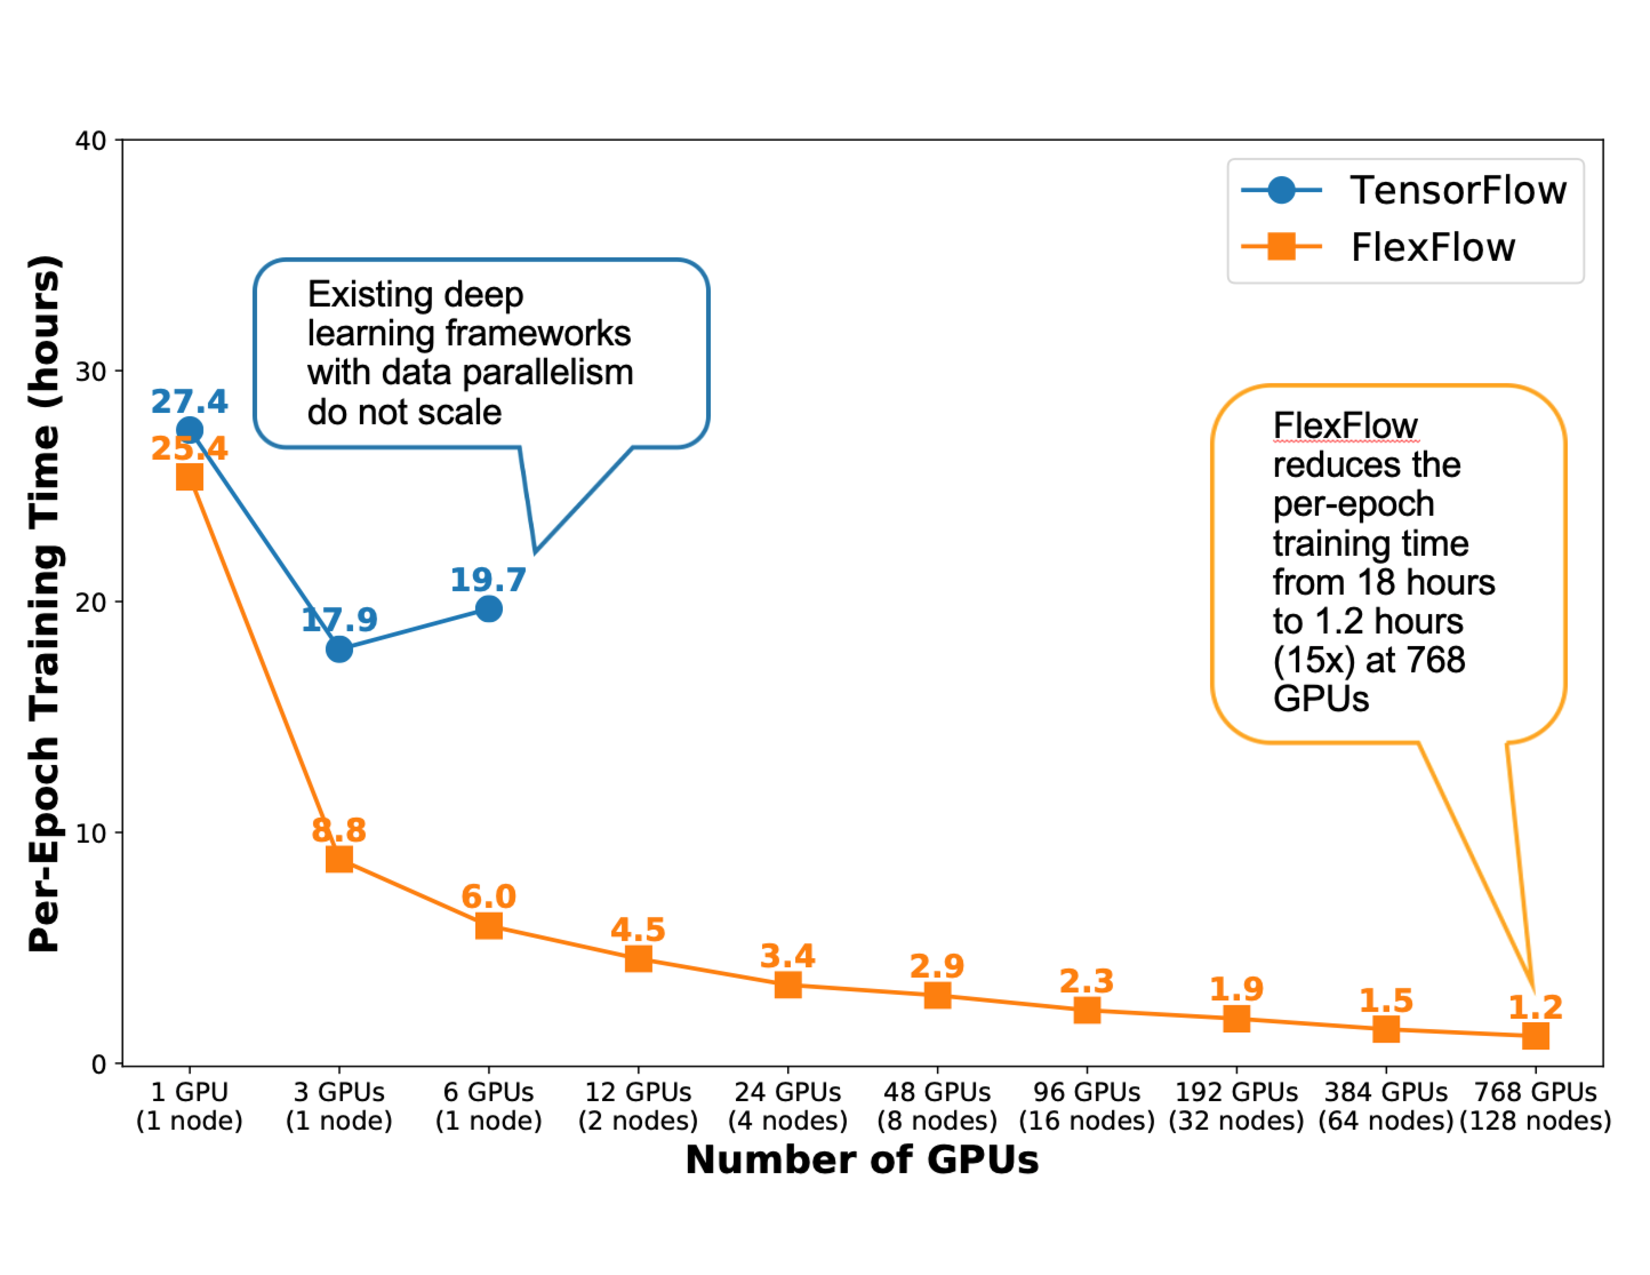
\includegraphics[width=0.6\textwidth]{projects/2.3.1-PMR/2.3.1.08-Legion/flexflow.pdf}
  \caption{The CANDLE project requires training and inference on large DNNs, which are 
    computationally intensive and difficult to parallelize. Training a single 
    epoch of the Uno dataset (with 21M samples) using TensorFlow requires 27 hours 
    on 1 GPU and 18 hours on 3 GPUs. Using FlexFlow,a deep learning framework built on 
    top  Legion, reduces training time to 1.2 hours on 128 Summit nodes (768 GPUs).
    The features enabling this are Legion’s first-class data partitioning, which enables
    more flexible and efficient parallelization strategies than are supported by 
    existing frameworks.
  }
  \label{fig:2.3.2.08:flexflow}   
\end{figure}

\paragraph{Next Steps}
Our plans for the next year are to continue focusing on the 
challenges presented by the upcoming exasacle system architectures 
and on hardening and improving the overall performance and scalability 
of Legion.  In addition to the Office of Science systems (Aurora and Frontier)
we will also consider support for the Sierra and El Capitan platforms at 
Lawerence Livermore to support NNSA components that are using Legion.  We will 
continue to seek out and improve our educational outreach and developer productivity, 
including regular open source releases of Legion and direct interactions with the 
applications teams for debugging, fine-tuning of features for particular use cases and 
overall performance tuning.  We are also actively interacting with a growing community of 
interested users from outside the traditional HPC community where data-centric and 
accelerated machine learning use cases are of growing importance.  
